\documentclass{article}
\usepackage{xeCJK}
\usepackage{amsmath}
\usepackage{listings}
\usepackage{xcolor}
\setlength{\parindent}{0pt}
\renewcommand{\baselinestretch}{1.0}
\lstset{
	frame=tb, % draw a frame at the top and bottom of the code block
	showstringspaces=false, % don't mark spaces in strings
	numbers=left, % display line numbers on the left
	commentstyle=\color{green}, % comment color
	keywordstyle=\color{blue}, % keyword color
	stringstyle=\color{red} % string color
}
\usepackage[a4paper,left=20mm,right=20mm,top=15mm,bottom=15mm]{geometry}  

\title{Catalan Number}
\author{MengChunlei}

\begin{document}
\maketitle
\section{题目描述}
有$n$个左括号'('以及$n$个右括号')'组成的所有排列中, 有多少个是合法的括号匹配(即任何前缀,左括号的个数不小于右括号). 令$f(n)$表示个数, 那么有$f(1)=1$, 即'()', $f(2)=2$, 即'()()'和'(())'.
\section{解决思路}
首先, 对这个问题做一个转化.初始时, 二维坐标的原点(0,0).左括号表示向$x$方向前进一个单位,即$(a,b)$到$(a+1,b)$.同理,右括号表示向$y$方向前进一个单位,即$(a,b)$到 $(a,b+1)$. 那么这个问题就转化为有多少条路径可以从$(0,0)$到$(n,n)$且路径都在$y=x$这条线的下方. \par
对于$n=4$,下面是一些合法的路径.\par
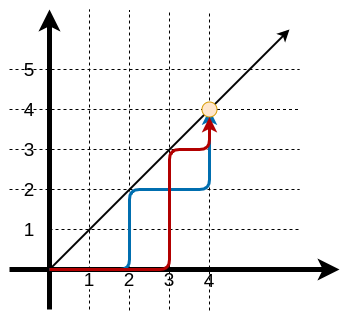
\includegraphics[scale=0.8]{pic1.png} \par

如果不考虑$y=x$的限制, 那么所有的路径有$\binom{2n}{n}$条. 然后考虑不合法的路径.对于一条不合法的路径, 如下图的蓝色实线所示, 它一定与直线$y=x+1$有一个交点(红点的位置),然后将这个交点之后一直到$(n,n)$之间的路径沿着$y=x+1$作翻转, 如蓝色虚线所示, 那么这条蓝色虚线的终点为$(n-1,n+1)$. \par
可以发现每一条不合法的路径, 按照这个翻转规则, 都对应一条从$(0,0)$到$(n-1,n+1)$的路径, 所以不合法的路径为$\binom{2n}{n+1}$. \par
所以$f(n)=\binom{2n}{n}-\binom{2n}{n+1}$\par
~\\
$=\frac{(2n)!}{n!n!}-\frac{(2n)!}{(n+1)!(n-1)!}$\par
~\\
$=\frac{1}{n+1}\left (\frac{(2n)!(n+1)}{n!n!}-\frac{(2n)!}{n!(n-1)!}  \right )$ \par
~\\
$=\frac{1}{n+1}\left (\frac{(2n)!(n+1)}{n!n!}-\frac{(2n)!n}{n!n!}  \right )$\par
~\\
$=\frac{1}{n+1}\frac{(2n)!}{n!n!}=\frac{1}{n+1}\binom{2n}{n}$\par
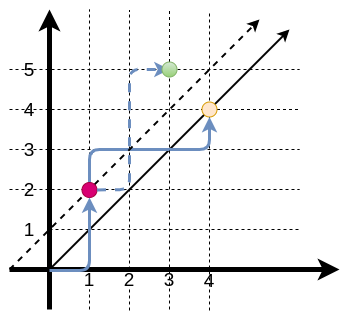
\includegraphics[scale=0.8]{pic2.png} \par

\section{总结}
这个数列叫做卡特兰数,$C_{n}$.它的前几项如下: \par
~\\
$\begin{matrix} 
C_{0} & C_{1} & C_{2} & C_{3} & C_{4} & C_{5} & C_{6} & C_{7} & C_{8} \\ 
1 & 1 & 2 & 5 & 14 & 42 & 132 & 429 & 1430 \\
\end{matrix}$ \par
~\\
还有一些其他的关系:
\begin{itemize}
	\item $C_{n+1}=\sum_{i=0}^{n-1}C_{i}C_{n-i}$
    \item $C_{n+1}=\frac{4n+2}{n+1}C_{n}$
    \item $\sum_{n\geq 0}\binom{2n}{n}\frac{z^{n}}{n+1}=\sum_{n\geq 0}C_{n}z^{n}=\frac{1-\sqrt{1-4z}}{2z}$
\end{itemize}
\end{document}
